\section{Results}

Using the methodology described above, I gathered the following results. Figure~\ref{fig:cpu-wall-child} on page~\pageref{fig:cpu-wall-child}, Figure~\ref{fig:io-wall-child} on page~\pageref{fig:io-wall-child}, and Figure~\ref{fig:mix-wall-child} on page~\pageref{fig:mix-wall-child} show the average wall time per child process averaged over three trial runs for the three different benchmarks.  Each figure shows the results for a specific benchmark and compares the performance of each scheduling policy based on number of child processes.

The CPU bound benchmark results in Figure~\ref{fig:cpu-wall-child} show that while the number of processes remains relatively low the SCHED\_OTHER scheduling policy out-paces the other policies tested; at high numbers of processes the advantage disappears for all intents and purposes.  Both of the Real-time scheduling algorithms perform relatively equally regardless of number of processes.  Additionally, as the number of processes increases, each process takes more time to complete.

%\begin{figure}[H]
\begin{figure}[hbtp]
  \centering
  \includegraphics[scale=0.8]{img/cpu-wall-child.eps}
  \caption{}
  \label{fig:cpu-wall-child}
\end{figure}

The I/O bound benchmark results in Figure~\ref{fig:io-wall-child} show that a higher priority scheduling algorithm improves wall time.  As the number of processes increases, the performance of the different scheduling algorithms converges and the amount of time for each process to complete decreases.

\begin{figure}[hbtp]
  \centering
  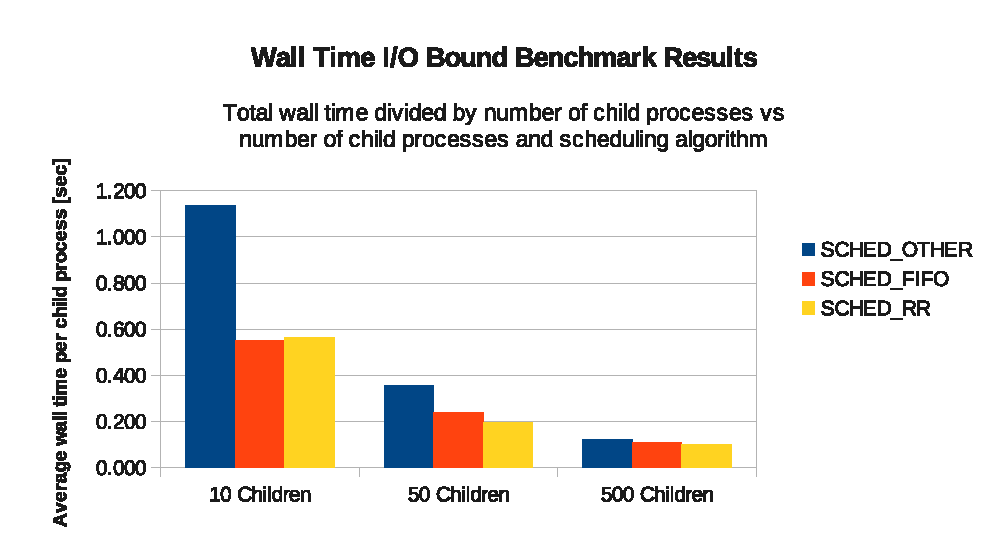
\includegraphics[scale=0.8]{img/io-wall-child.eps}
  \caption{}
  \label{fig:io-wall-child}
\end{figure}

The mixed benchmark results in Figure~\ref{fig:mix-wall-child} show that the scheduling policy does not have a significant impact on the amount of time each process takes to complete execution.  As the number of processes increases, the amount of time each process takes to complete its execution decreases.

\begin{figure}[hbtp]
  \centering
  \includegraphics[scale=0.8]{img/mix-wall-child.eps}
  \caption{}
  \label{fig:mix-wall-child}
\end{figure}
